\documentclass{article}

\usepackage[spanish]{babel}
\usepackage[utf8]{inputenc}

\usepackage{graphicx}
\graphicspath{{./../imgs/}{./../../../imgs/}}

\usepackage{geometry}
\geometry{a4paper, margin=1in}

\usepackage{fancyhdr}
\setlength{\headheight}{28.2pt}

\usepackage{listings}

\title{\vspace{-30pt}Laboratorio 2: Implementación de filtros}
\author{Gonzalo G. Fernández}
\date{\today}

\begin{document}

\pagestyle{fancy}
\fancyhead{}
\fancyhead[C]{\Large Diseño Digital Avanzado}
\lhead{
\includegraphics[height=0.8cm]{logo_ff.png}}

\maketitle
\thispagestyle{fancy}

\section*{Efectos de cuantización}

Ejecutar los script de python con el objetivo de comprender los efectos de cuantización de los coeficientes.

\begin{itemize}
    \item fir\_filter\_direct\_form.ipynb
    \item iir\_filter\_direct\_form.ipynb
    \item IIR\_Filter\_Design.ipynb
\end{itemize}

Instanciar y ejecutar el testbench de cada uno de los filtros.

\begin{itemize}
    \item filtro\_fir.v, tb\_filtro\_fir.v
    \item iir.v, filter\_tb.v
    \item iir\_top.v, iir\_filter.v, coeffSec1.v, coeffSec2.v, coeffSec3.v, tb\_iir\_filter.v
\end{itemize}

Los resultados de las simulaciones de las Fig. \ref{fig:tb_filtro_fir}, \ref{fig:filter_tb} y \ref{fig:tb_iir filter}.

\begin{figure}[ht]
    \centering
    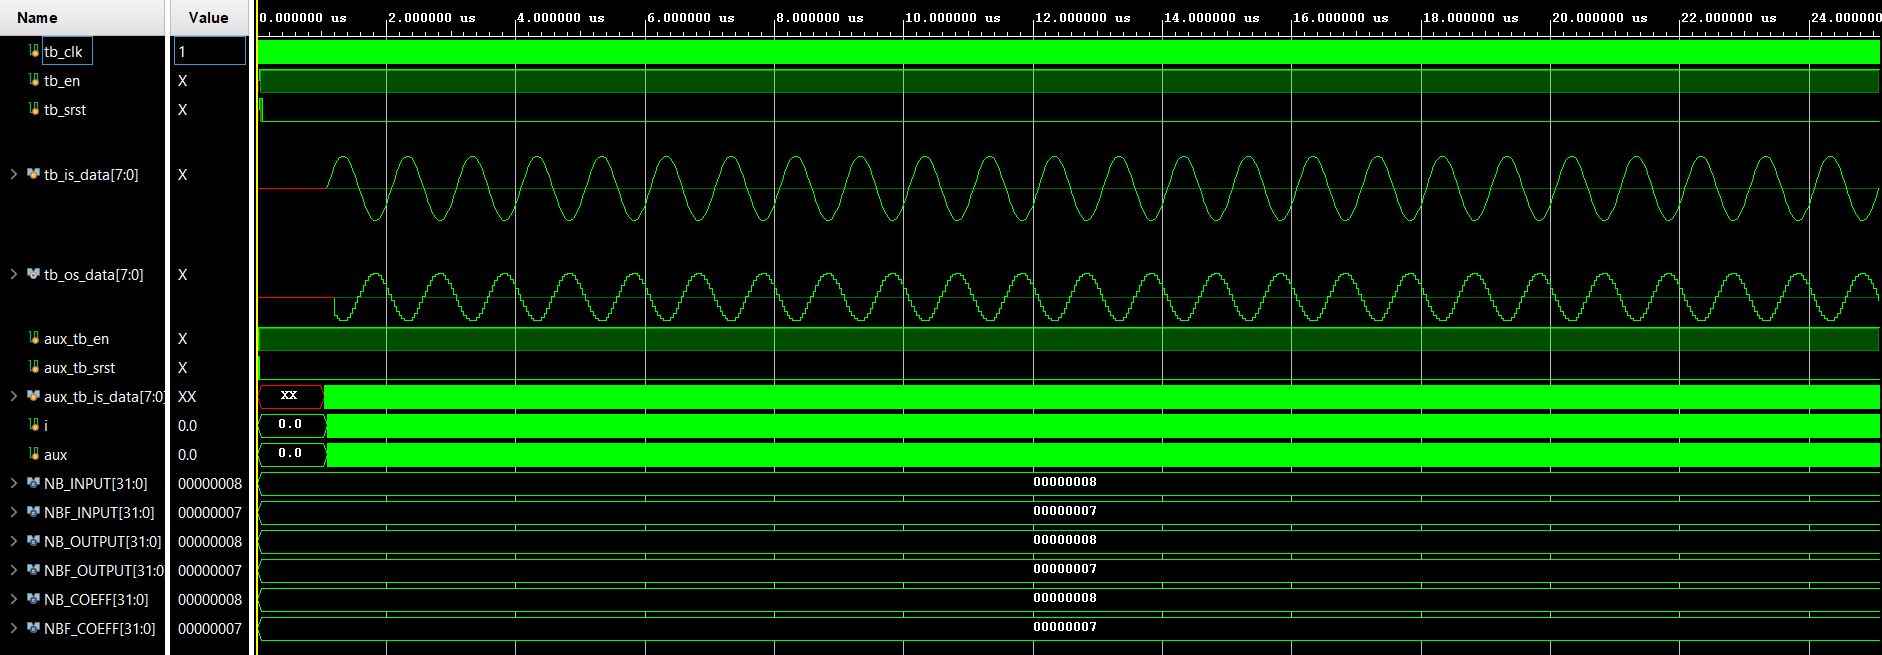
\includegraphics[width=\textwidth]{sim-tb_filtro_fir.jpg}
    \caption{Forma de onda obtenida del testbench tb\_filtro\_fir.v}
    \label{fig:tb_filtro_fir}
\end{figure}

\begin{figure}[ht]
    \centering
    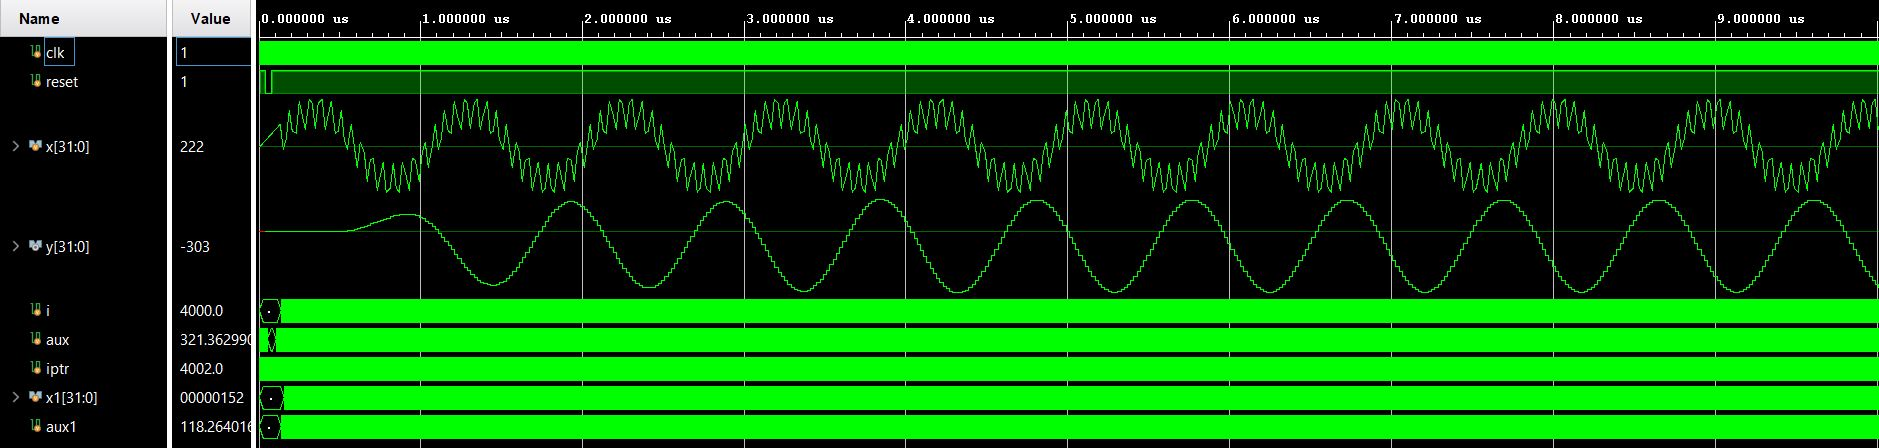
\includegraphics[width=\textwidth]{sim-filter_tb.jpg}
    \caption{Forma de onda obtenida del testbench filter\_tb.v}
    \label{fig:filter_tb}
\end{figure}

\begin{figure}[ht]
    \centering
    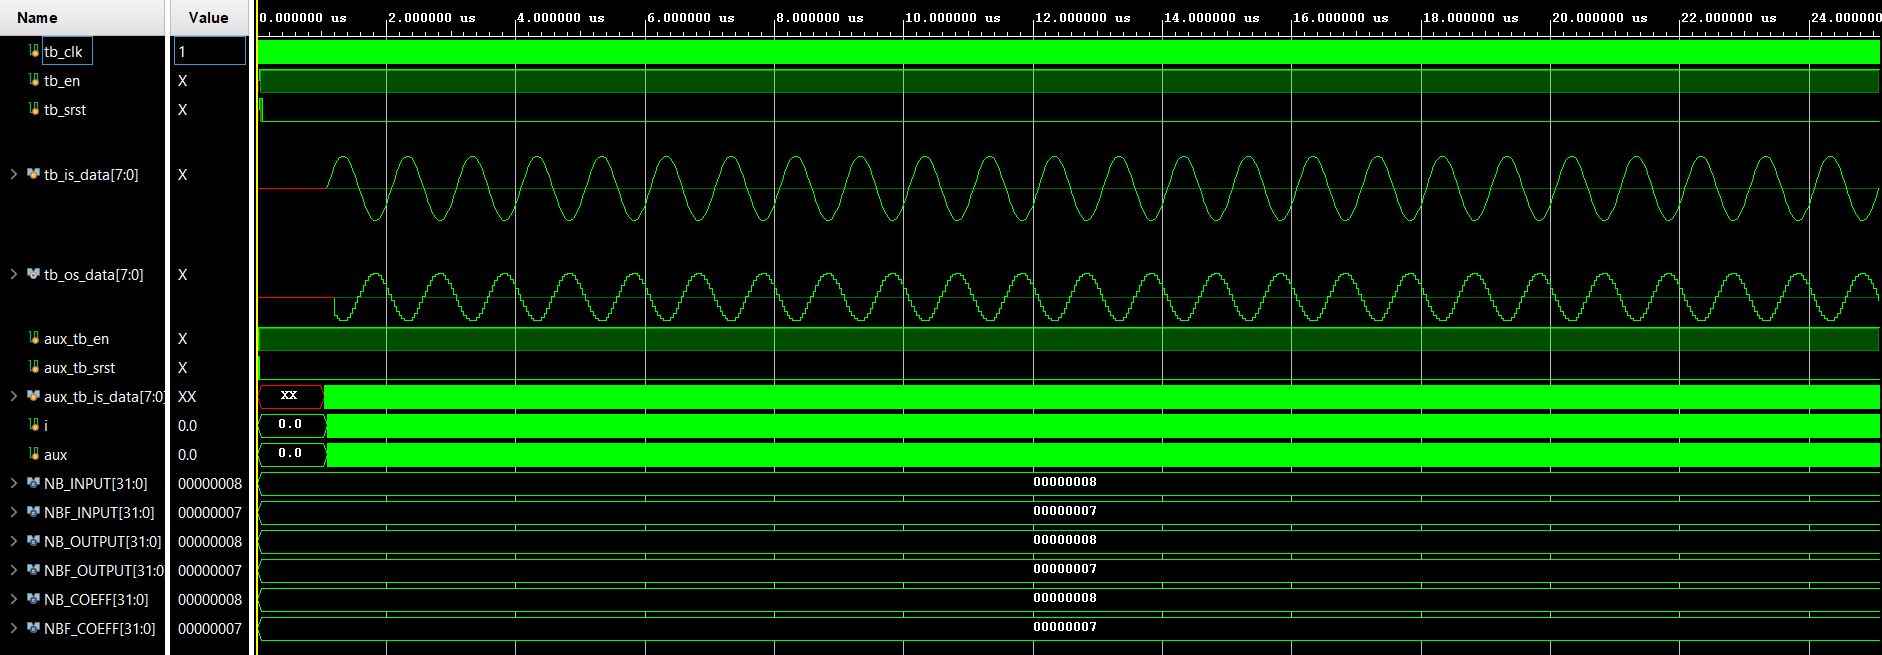
\includegraphics[width=\textwidth]{sim-tb_filtro_fir.jpg}
    \caption{Forma de onda obtenida del testbench tb\_iir\_filter.v}
    \label{fig:tb_iir filter}
\end{figure}

\section*{Primer modelo}

Implementar en FPGA el filtro FIR según los siguientes archivos:

\begin{itemize}
    \item top\_design.v
    \item signal\_generator.v
    \item filtro\_fir.v
    \item SatTruncFP.v
\end{itemize}

Agregar los IPs VIO e ILA para controlar en forma remota el diseño.

\section*{Laboratorio}

Considerar un sistema de transmisión compuesto por una señal senoidal y un filtro pasa bajo con las siguientes características:

\begin{itemize}
    \item Señal senoidal compuesta por dos frecuencias $f_{1} = 17 kHz$ ($A=0.5$) y $f_{2} = 1.5 kHz$ ($A=1.0$)
    \item Frecuencia de muestreo $f_{s} = 48 kHz$
    \item Filtro pasa bajo con frecuencia de corte $f_{cut} = 8 kHz$
\end{itemize}

Desarrollo del modelo:

\begin{enumerate}
    \item Utilizando el script de python coeff.ipynb, determinar los coeficientes del filtro para una frecuencia de corte de $f_{cut} = 8 kHz$. El filtro debe tener una longitud de 15 coeficientes.
    \item Realizar el diagrama de bloques del filtro (Fig. \ref{fig:block-diag}).
    \item Generar un proyecto con los archivos entregados por la cátedra con la herramienta Vivado.
    \item Configurar el archivo mem.hex con las señales senoidales especificadas previamente utilizando el script genmem.py.
    \item Generar los coeficientes del filtro en Verilog con los valores de los coeficientes cuantizados (sintetizar cada filtro por separado).
    \item Implementar en FPGA y graficar las señales senoidales pre y pos filtradas (Fig. \ref{fig:filter05}, \ref{fig:filter8} y \ref{fig:filter18}).
\end{enumerate}

\begin{figure}[ht]
    \centering
    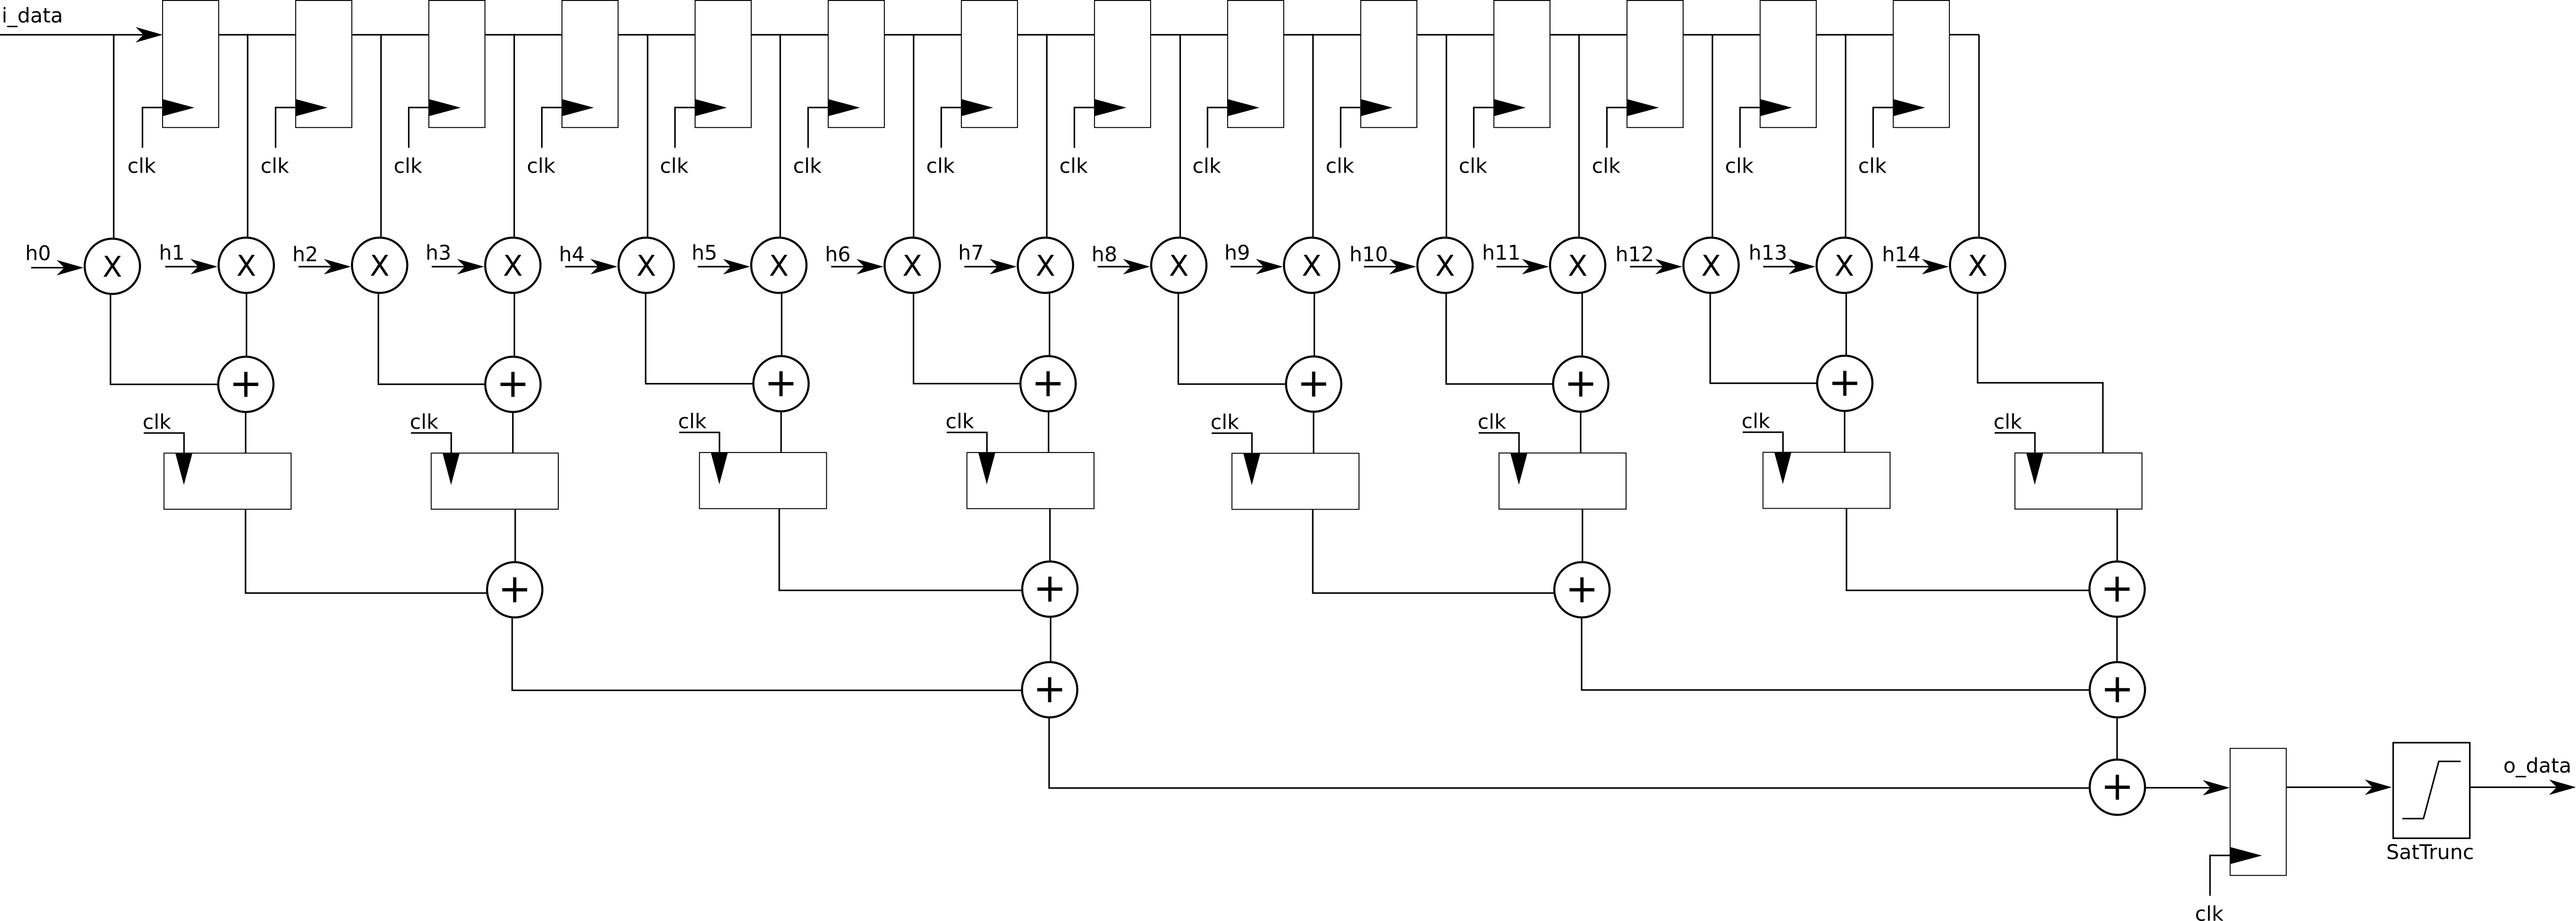
\includegraphics[width=\textwidth]{block_diag.png}
    \caption{Diagrama de bloques del filtro}
    \label{fig:block-diag}
\end{figure}

\begin{figure}[ht]
    \centering
    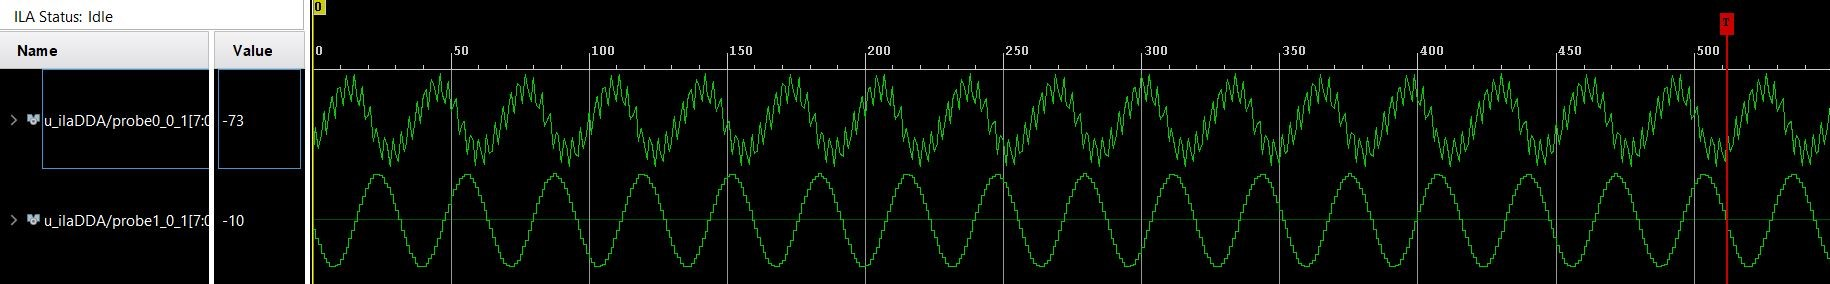
\includegraphics[width=\textwidth]{impl-cutoff_0_5khz.jpg}
    \caption{Forma de onda obtenida de ILA con implementación de filtro con frecuencia de corte $0.5 kHz$}
    \label{fig:filter05}
\end{figure}

\begin{figure}[ht]
    \centering
    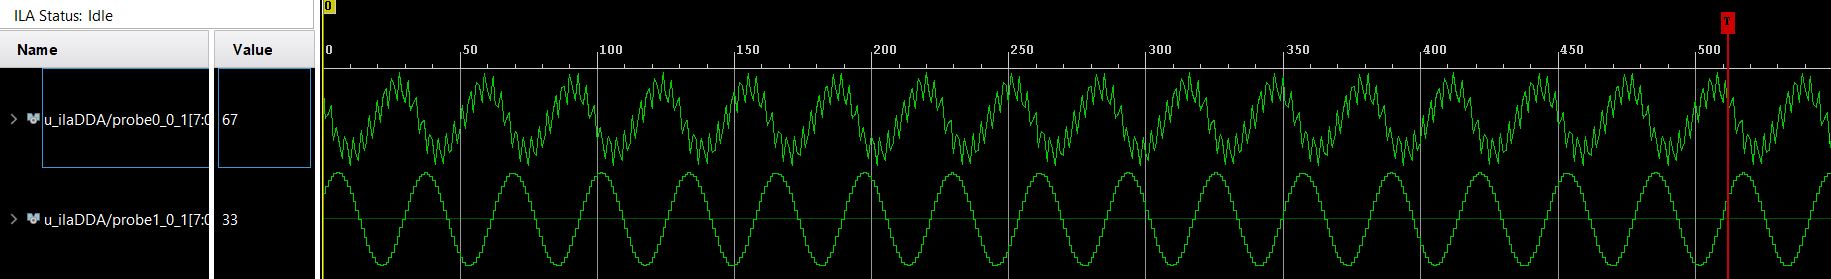
\includegraphics[width=\textwidth]{impl-cutoff_8khz.jpg}
    \caption{Forma de onda obtenida de ILA con implementación de filtro con frecuencia de corte $8 kHz$}
    \label{fig:filter8}
\end{figure}

\begin{figure}[ht]
    \centering
    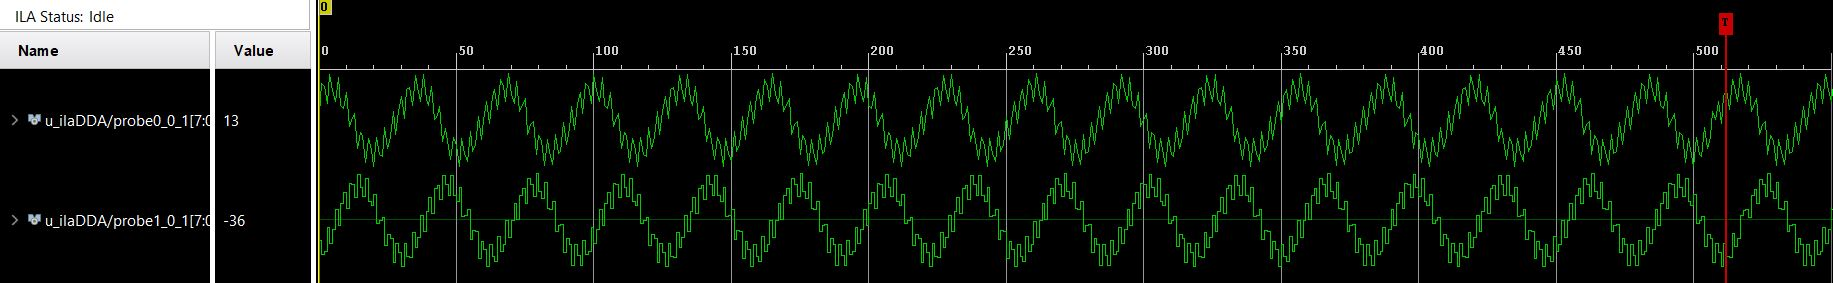
\includegraphics[width=\textwidth]{impl-cutoff_18khz.jpg}
    \caption{Forma de onda obtenida de ILA con implementación de filtro con frecuencia de corte $18 kHz$}
    \label{fig:filter18}
\end{figure}

\end{document}